\chapter{Applications}
\label{ch:Applications}
In this chapter, we will introduce basic implementations and applications of Continuous Hopfield Neural Networks. The results of the contents of this chapter are replicable using the open source repository \cite{github_repo}. We recall contents, techniques and interpretations of the course notes of Deep Learning and Applied Artificial Intelligence of \citet{DLAI}.

\section{Implementations}
In \cref{def:updating}, we defined the updated state of a Hopfield neural network as:
\[
\xi^{\text{new}} = X \softmax \left(\beta X^T \xi\right)
\]
This neural network is used to classify inputs, so it is more informative to study the evolution of the logits. A \textbf{logit} represents the degree to which an input adheres to a particular feature. For example, the image of a '$1$' may resemble that of a '$7$', meaning that the '$1$' may have a high logit for feature '$7$'. Typically, the softmax of all logits represents the probability that the $1$ is classified as a $7$ in this case. Note that the vector of logits is proportional to the vector of magnetisations for each pattern, in particular $l_\mu = N\beta m_{N,\mu}(\xi)$ from \cref{def:mattis_mgn}.

\noindent An equivalent way to express the update formula using logits is
\[
l^{\text{new}} = \beta X^T \xi^{\text{new}} = \beta X^T X \softmax \left(l\right)
\]
We define $A_\beta \mathdef \beta X^T X$, so $l^{\text{new}} = A_\beta \softmax \left(l\right)$. A Hopfield neural network can be thought of as a cyclic \texttt{FCL} with softmax activation:

\begin{figure}[htbp]
	\centering
	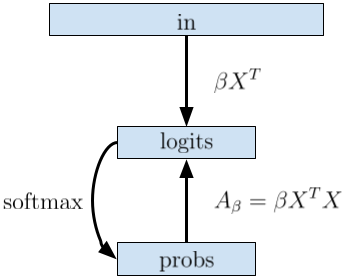
\includegraphics[width=0.4\linewidth]{Figures/FCL.png}
	\caption{Diagram of the Hopfield neural network. The input (on the top) passes through a fully connected layer with parameters $\beta X^T$ and zero bias. The logits are then fed into a cyclic loop, and the output is obtained. To reconstruct the image, we can use the \textit{probs} layer; $Xp=\xi$, so we can connect an FC layer without bias and weights $X$ to the \textit{probs} layer.}
	\label{fig:FCL}
\end{figure}

\paragraph{Convolutions} A Hopfield neural network looks at the whole image and analyses the image as a whole. To restrict the analysis to a smaller Hopfield neural network, we can define a convolution of the Hopfield neural network. This allows us to reconstruct small patterns in more small parts of the image. A convolution returns a new image with more (or less) channels with logits, and each logit indicates the presence of a pattern in the image.

\noindent Let $H$ be a Hopfield neural network that takes $C_i \times S$ neurons as input and returns $C_o$ logits, where $S$ is a shape (e.g. $3 \times 3$) with $n$ dimensions. A convolution applies $H$ to each region of shape $S$ in data with $C_i$ channels and $n$ dimensions.

\noindent For example, if we have an image of size $32 \times 32$ with $3$ channels (\texttt{RGB}), we can apply a convolution with a $4 \times 4$ filter. In this case $H$ operates on $3 \times 4 \times 4 = 48$ neurons and detects $5$ patterns. The convolution returns data with $5$ channels and a shape of $29 \times 29$, where each position represents the response to a pattern for that region of the image.

\noindent In \cref{fig:CNN} we can see that a convolution works in a similar way to a classical Hopfield neural network.
\begin{figure}[htbp]
    \centering
    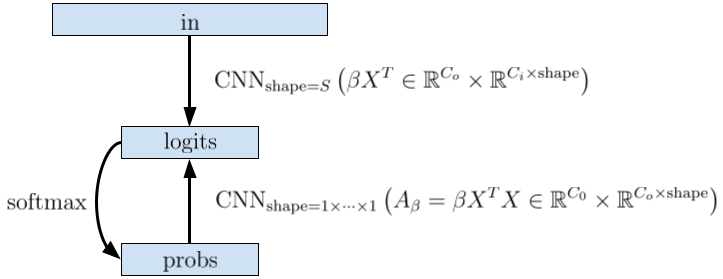
\includegraphics[width=0.8\linewidth]{Figures/CNN.png}
    \caption{The neural network receives data in the form of $C_i \times S$. A convolutional layer computes the logit vector for each region, producing data in the form of $C_o \times S$. A pointwise softmax is then applied to each logit vector. Finally, each logit vector is linearly transformed and a pointwise convolutional layer is applied, producing data of the form $C_o \times S$.}
    \label{fig:CNN}
\end{figure}

\begin{remark}[Generalized Continuous Hopfield Neural Networks]
	During training, the parameters of a Hopfield neural network can become difficult to interpret. Is it possible to train a number of parameters that is not directly proportional to the number of neurons?

	\noindent The matrix $A_\beta$ is not arbitrary. In fact, it must satisfy the following properties:
	\begin{itemize}[itemsep=2pt, topsep=10pt]
		\item $A_\beta$ is a real, square, and symmetric matrix.
		\item $A_\beta$ is non-negative: $v^T A_\beta v = \beta v^T X^T X v = \beta \|Xv\|^2 \geq 0$.
	\end{itemize}
	Therefore, if interpretability is not an issue, we can train over a matrix $M \in \mathbb{R}^{C \times C}$ and set $A_\beta = M^T M$. In this way the Hopfield neural network can be seen as a composition of: a \texttt{FC} layer with parameter $\beta X^T$ and bias $0$, a cycle with $A_\beta = M^T M$, and another \texttt{FC} layer with parameter $X$ and bias $0$.

	\noindent This observation also applies to convolutional Hopfield nets.
\end{remark}

\paragraph{Autoencoders}
Note that the number of parameters $P$ is much smaller than the number of neurons $N$, so image reconstruction using Hopfield neural networks is a special case of \textbf{autoencoder}. In fact, the Hopfield neural network reduces the dimensionality of the input (with $N$ neurons), then it recalls the pattern in the loop and reconstructs the image from it, in detail:
\[
XH_{\beta,X}\left(\xi\right) = XH_{A_\beta}'\left(\beta X^T\xi\right)
\]
where $H$ is the main Hopfield neural network with $N$ neurons and $P$ patterns, $H'$ is a Hopfield neural network with $P$ neurons and $P$ patterns. $\beta X^T$ makes the code of $\xi$ (encoding), this code is cleaned in the loop (in a manifold) and finally it is rebuilt (decoding).

\noindent Now we derive a variational autoencoder from Hopfield neural networks and \textit{PCA}. We observe that a Hopfield neural network is a variant of a \textit{PCA} because it uses a matrix and its transpose to encode and decode information, the only difference being an additional softmax layer, an internal loop, and an initial and final multiplicative constant\footnote{For more about PCA, see \url{https://www.cs.umd.edu/class/spring2019/cmsc422-0101/materials/lecture20-sp19.pdf}}. So we get a \textit{PCA} similar to a Hopfield net:
\begin{itemize}
    \item \textbf{encoding} : The input is multiplied by $\sqrt{\beta}X^T$.
    \item \textbf{decoding} : The code is multiplied by $\sqrt{\beta}X$.
\end{itemize}
Now we turn this autoencoder into a variational autoencoder. So the encoder returns information about some probability distribution and the decoder samples from that distribution and reconstructs the input, this is a \textbf{VAE}\footnote{For more about VAEs, see \url{https://www.ibm.com/think/topics/variational-autoencoder}}. We can see that a Hopfield neural network has the same architecture, but it has no sampling. The final architecture is shown in \cref{fig:VAE}.
\begin{figure}[htbp]
    \centering
    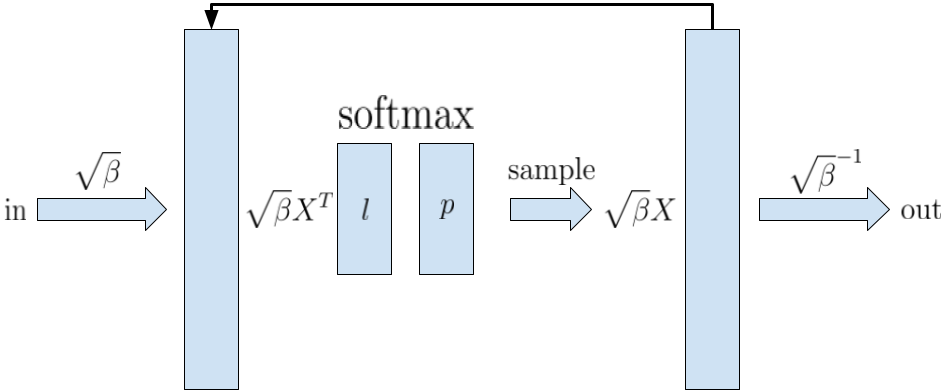
\includegraphics[width=0.9\linewidth]{Figures/VAE.png}
    \caption{The input is passed to the autoencoder with a simple multiplication ($\sqrt{\beta}$), then the autoencoder multiplies its input by $M^T$, this produces a vector of $P$ logits $l$, after a softmax we get a discrete distribution $p$. Now it's possible to simulate this distribution with one or more samples. This distribution is then passed to the decoder which multiplies it by $M$. This is a single loop and we can answer it using the output as a new input.}
    \label{fig:VAE}
\end{figure}

\section{DeepHNN}
First, we define a simple use of Hopfield neural networks. A \textbf{DeepHNN} is a Hopfield neural network with more patterns given the number of target features. In fact, using $3$ patterns per feature may be better than using only one pattern per feature. Thus, the logit returned by a DeepHNN is the maximum logit for any subset of patterns returned by a Hopfield neural network.

\begin{figure}[ht]
    \centering
    \begin{minipage}{0.45\textwidth}
        \centering
        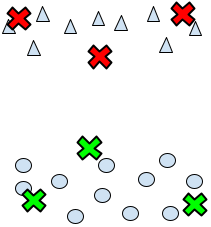
\includegraphics[width=0.6\linewidth]{Figures/DeepHNN.png}
    \end{minipage}
    \hfill % Spazio orizzontale tra le figure
    \begin{minipage}{0.45\textwidth}
        \centering
        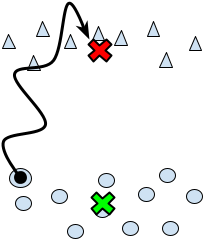
\includegraphics[width=0.6\linewidth]{Figures/DeepHNN_1.png}
    \end{minipage}
    \caption{We have two features: triangles and circles. By using $3$ patterns per feature, we can better capture the data with better coverage. However, the result may be more confusing.}
    \label{fig:DeepHNNDiagram}
\end{figure}

\noindent We have added a \textbf{final bias} for each pattern in the same feature. The bias can assign a confidence about a feature, it is very useful to interface with other layers. In a classical Hopfield neural network the bias is the same for each feature, but when there are other layers and in a more complex neural network it is better to add a new degree of freedom. In algorithm \ref{alg:HNN_forward} we show an excerpt of the code used for the forward pass. In particular, the implemented class \texttt{DeepHNN} uses more channels, a separate neural network for each channel.

\newpage

\begin{lstlisting}[style=code, label=alg:HNN_forward, caption=DeepHNN forward pass, language=Python]
import torch
from torch import nn
from torch.nn import functional

""" method of DeepHNN
attributes:
    iterations: int
    channels, features, deep, neurons: int
        positive values
    _logbeta: nn.Parameter
        with shape (channels,)
    _bias: nn.Parameter
        with shape (channels, features,)
    _patterns: nn.Parameter
        with shape (channels, deep * features, neurons,)
"""
def forward(self, x: torch.Tensor) -> torch.Tensor:

    # Shape of x must be (batch, channels, neurons)

    L = torch.exp(self._logbeta).view(self.channels, 1, 1) * self._patterns
    A = torch.einsum('cin , cjn-> cij', L, self._patterns)  # i,j are logits

    # main algorithm
    x = torch.einsum('cln, bcn -> bcl', L, x)  # get logits
    for _ in range(self.iterations):
        x = functional.softmax(x, dim=2)  # get probs
        x = torch.einsum('clp, bcp -> bcl', A, x)  # get logits

    # max reduction
    x = x.view(-1, self.channels, self.features, self.deep)
    x = torch.max(x, dim=3).values
    x = x + self._bias.view(1, self.channels, self.features)

    return x
\end{lstlisting}

\paragraph{A Simple Experiment}
The first experiment applies a Hopfield neural network with predefined patterns directly to an MNIST image. We manually define $3$ patterns for each digit between $0$ and $9$, and then implement a Hopfield neural network over $32 \times 32$ neurons. In \cref{fig:SimpleExp} we observe that the neural network has trouble recognizing the true digit. To solve this problem, we can try to train the neural network on MNIST and then analyze the results.

\begin{figure}[htbp]
    \centering
    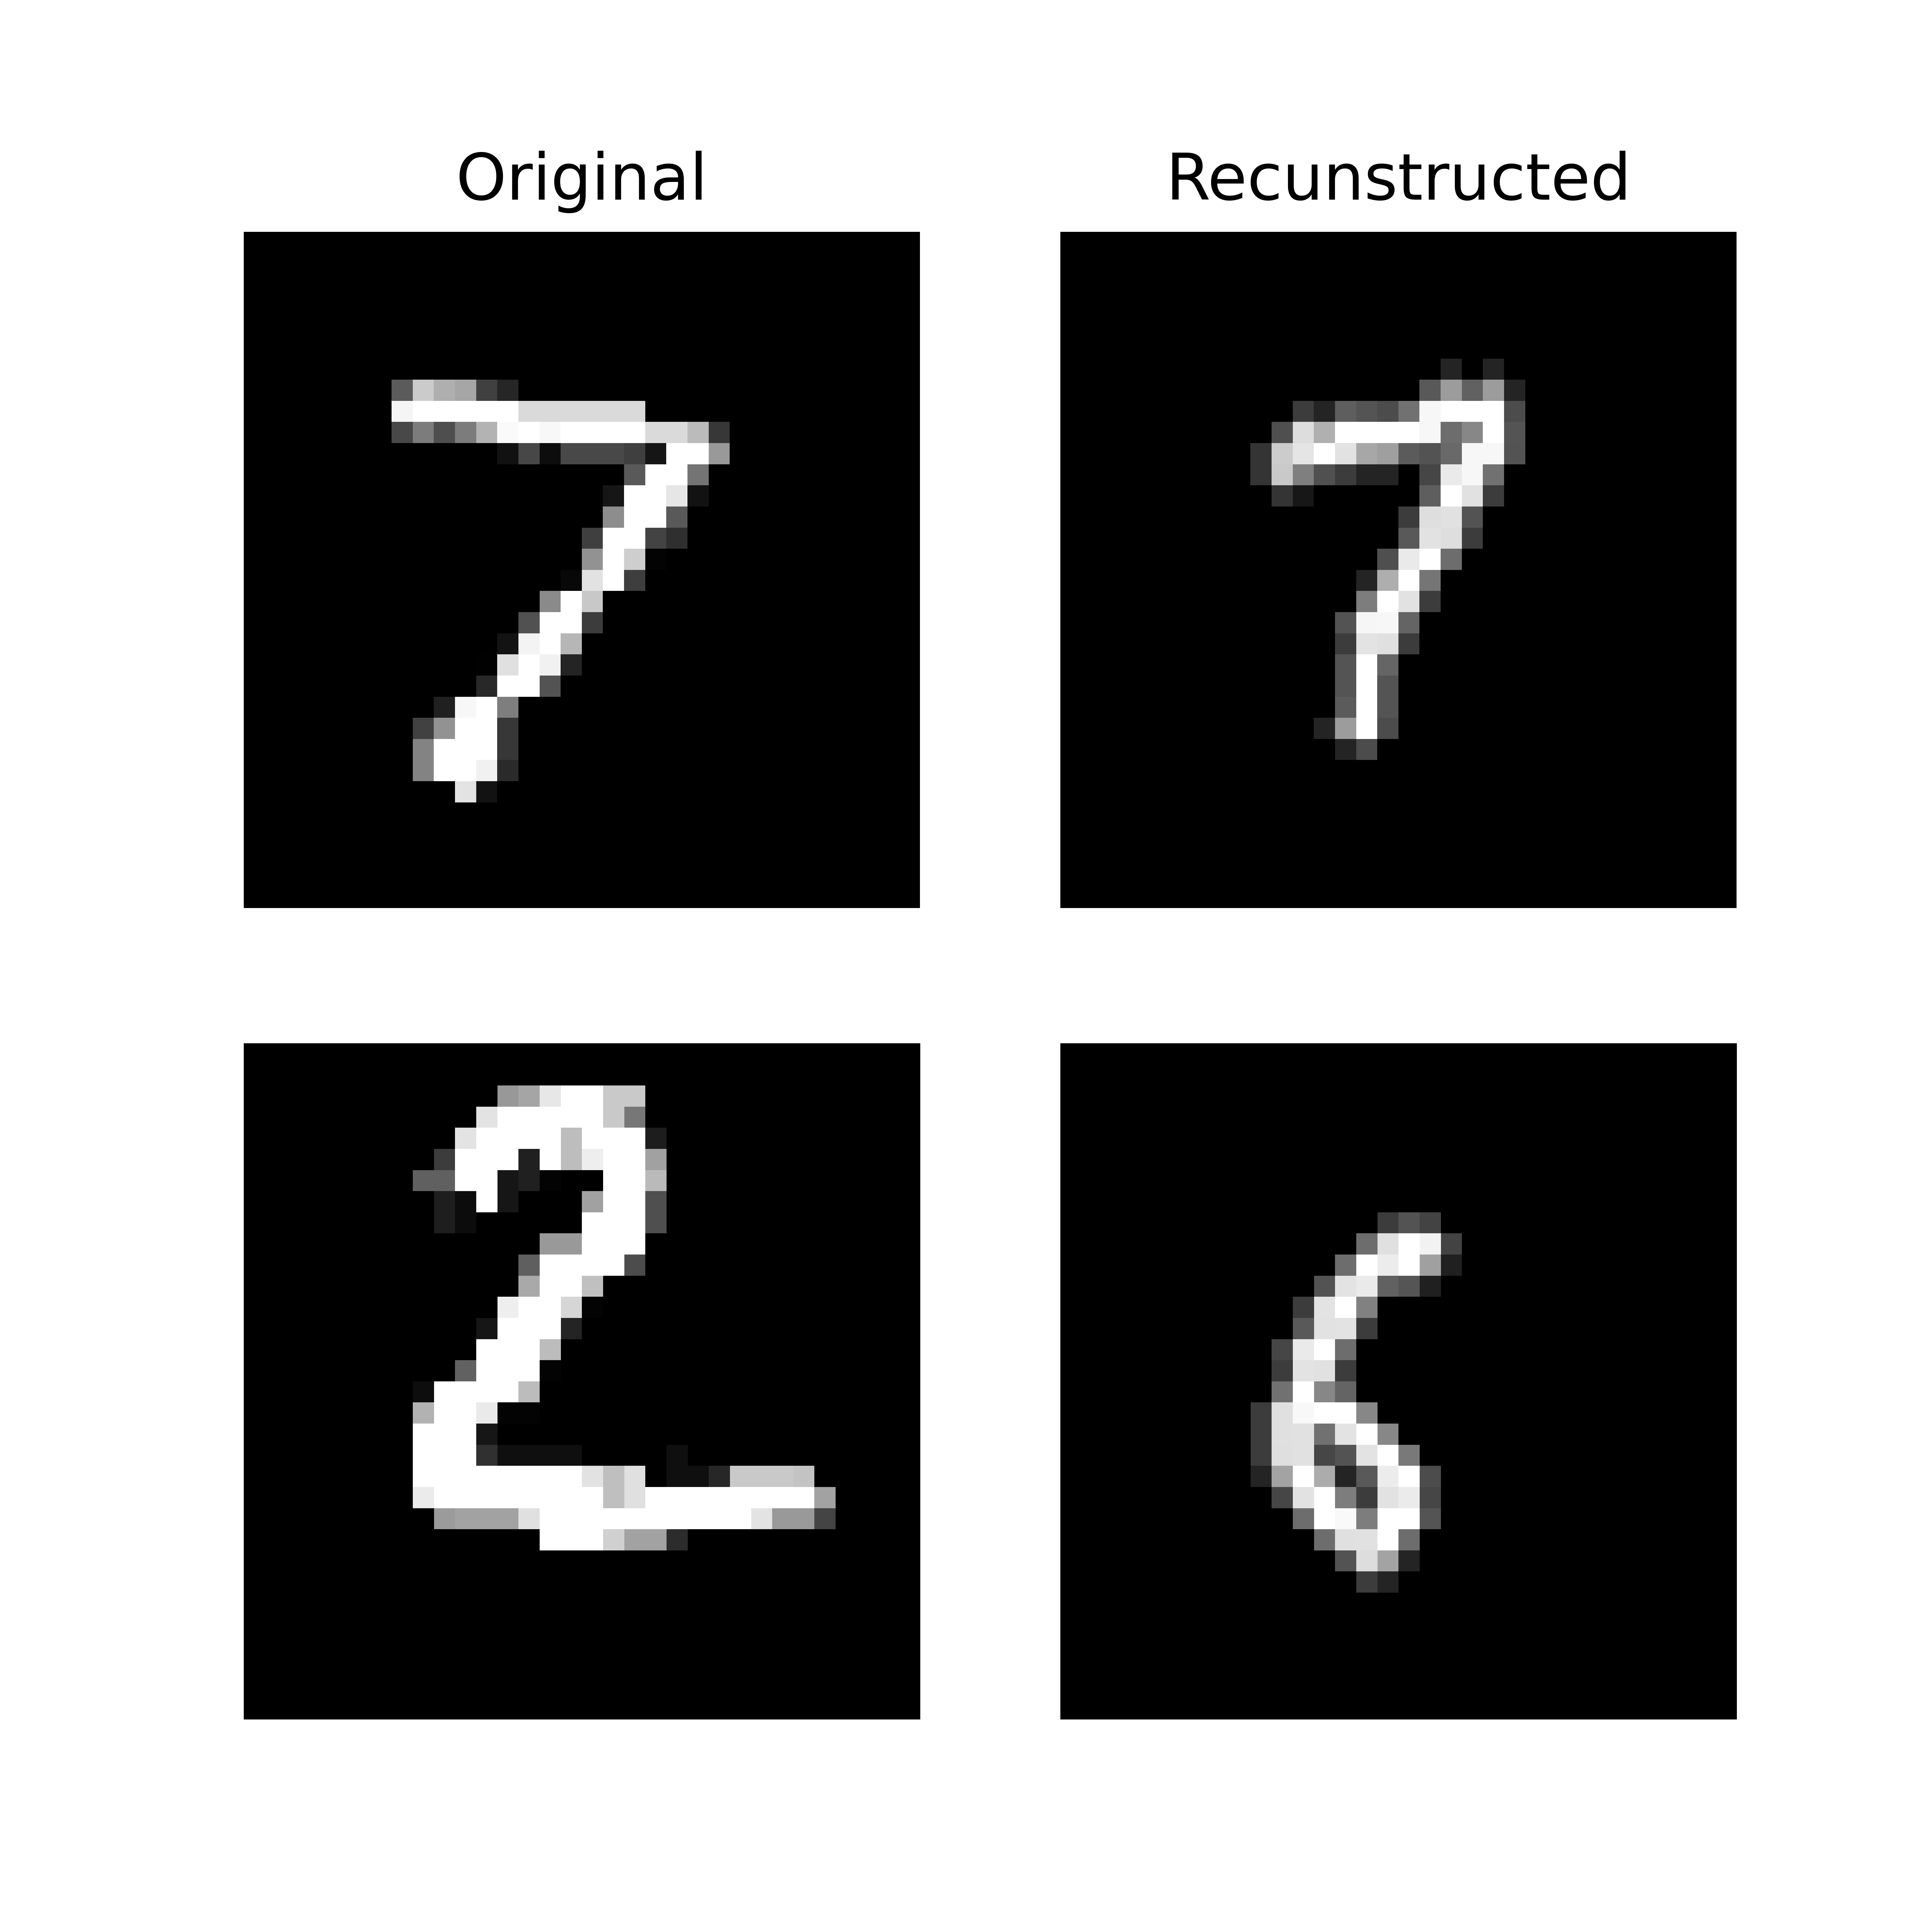
\includegraphics[width=0.5\linewidth]{Figures/SimpleExp.png}
    \caption{Applying a Hopfield neural network to two MNIST images. The Hopfield neural network had $\beta = 0.07$ and ran for 2 iterations.}
    \label{fig:SimpleExp}
\end{figure}

\noindent The neural network was trained using the cross-entropy loss for $40$ epochs with an adaptive learning rate using the current accuracy. At the end of training, the cross-entropy loss was $1.8$, and in the test phase, the neural network showed $32\%$ accuracy. The patterns with high attribution influence were not changed.

\paragraph{DeepHNN as MLP}
A single Hopfield neural network with the whole image as input is often not the best choice, because the output of the neural network depends entirely on the dot product with the vector patterns, i.e. moving all the pixels to the right (or left, or up, or down) will give a completely different output. Furthermore, we can observe that within a Hopfield neural network there is no notion of locality, in fact patterns are retrieved if and only if they are in the same position of the stored patterns. To overcome these problems, we observe that more smaller neural networks are better than only one, because they can analyze a small part of the images.

\noindent A convolution can create more "versions" of the same image, in particular it highlights a set of patterns in the image. For example, a convolution that detects horizontal lines and vertical lines will show, with high values, where there are horizontal lines and vertical lines. Thus, a single-channel image becomes a multichannel image (one for each feature). In addition, the number of patterns is usually not too large in relation to the number of input channels and the size of the kernel. Typically, the number of patterns is a quarter of the number of neurons in a kernel (e.g., $8$ input channels, $4\times4$ kernel size, $32$ output channels).

\noindent We define a neural network with a linear CNN that has $5$ channels with $4\times4$ kernels and $2$ steps. Then we use a DeepHNN with $5$ channels and $10$ features with deep $5$. Finally, we add a trainable convex reducer that merges all channels into only one and obtains $10$ logits. This neural network has $\num{56440}$ trainable parameters. We trained this neural network for $40$ epochs with a learning rate of $0.01$: the final accuracy obtained is $\approx87\%$ with a cross entropy loss of $0.7$. In \cref{fig:asMLP} it's possible to see details about the training, but kernels and patterns are not visible.

\begin{figure}[htbp]
    \centering
    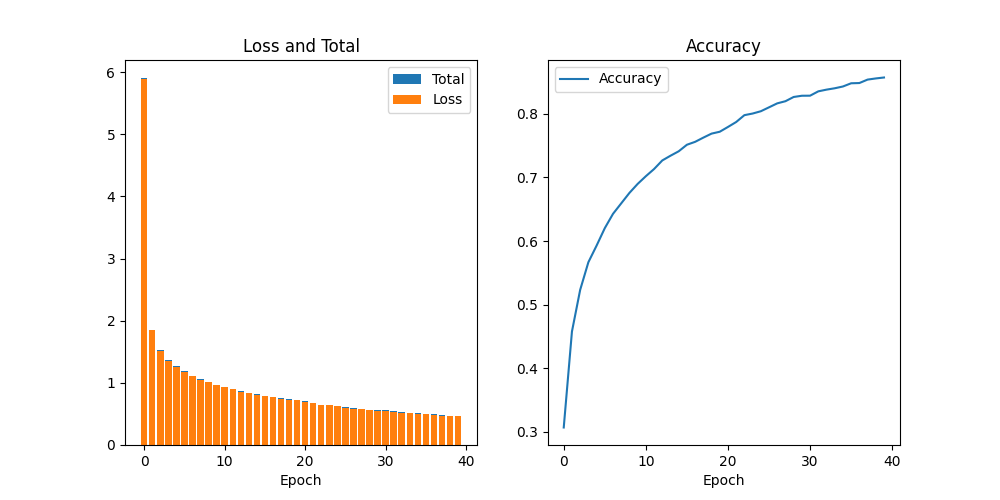
\includegraphics[width=0.9\linewidth]{Figures/asMLP.png}
    \caption{On the left the loss evolution during training (in orange the cross entropy loss, in blue the part due to the regularization), on the right the accuracy evolution.}
    \label{fig:asMLP}
\end{figure}

\section{ConvHNN2d}
We define a convolutional layer with Hopfield as a small Hopfield neural network that detects patterns in all parts of the image (see \cref{fig:CNN}). In this experiment, we use a $2d$ convolution to use over MNIST.

\noindent The main difference between a typical linear convolution and this convolution is how it highlights the patterns. A linear convolution pattern works over logits, so if it looks for the pattern $\left(1,1\right)$, it will highlight the pattern $\left(5,5\right)$ with value $10$ (excellent compatibility) and the pattern $\left(1,1\right)$ with value $2$ (good, but not excellent). So it works not in terms of distance, but in terms of the scalar product (intensities and directions) of patterns. A Hopfield neural network looks at patterns in a different way and does not work in terms of distance or scalar products. The Hopfield neural network tries to recall a pattern so that the final image is a mixture of recalled patterns for each region of the image, so it can clean the image from noise, and this behaviour is very useful when this neural network is the first convolutional layer. In the algorithm \ref{alg:CNN_forward} we show the forward pass of this layer.

\newpage
\begin{lstlisting}[style=code, label=alg:CNN_forward, caption=ConvHNN2d forward pass, language=Python]
import torch
from torch import nn
from torch.nn import functional

""" method of ConvHNN2d
attributes:
    channels_in, channels_out: int
        positive values
    kernel_size, padding, stride, dilation
        parameters of classical convolution
    iterations: int
        number of neurons of theoretical Hopfield neural network
    _logbeta: nn.Parameter
        with shape (1,)
    _bias: nn.Parameter
        with shape (channels_out,)
    _patterns: nn.Parameter
        with shape (channels_out, channels_in, kernel_size)
"""
def forward(self, x: torch.Tensor) -> torch.Tensor:

    # Shape of x must be (batch, channels_in, #, #)

    weight_loop = (
        torch.exp(self._logbeta)
        * torch.einsum(
            'in, jn -> ij',  # i,j are logits (channels_out)
            self._patterns.view(self.channels_out, -1),
            self._patterns.view(self.channels_out, -1)
        )
    ).view(self.channels_out, self.channels_out, 1, 1)

    x = nn.functional.conv2d(
        x,
        torch.exp(self._logbeta) * self._patterns,
        stride=self.stride,
        padding=self.padding,
        dilation=self.dilation,
    )
    for _ in range(self.iterations):
        x = nn.functional.softmax(x, dim=1)
        x = nn.functional.conv2d(x, weight_loop)

    return x + self._bias.view(1,self.channels_out,1,1)
\end{lstlisting}

\noindent In this experiment, we define a simple neural network that attempts to reconstruct an image using only convolutions. In particular, the input image has Gaussian noise, so we will use ConvHNN2d to remove the noise and reconstruct the original image. A Hopfield convolution produces an image with $C_{\text{out}}$ logits per pixel, so for each vector of logits per pixel we can recall the pattern using this formula:
$$
    \text{recalled pattern} = X\softmax\left(\text{logits}\right)
$$
Thus, the transposed convolution combines all the reconstructed patterns and obtains an approximation of the original convolution. In our architecture, a ConvHNN2d uses $9$ patterns with kernel size $(5,5)$. Thus, it produces a new image with $9$ channels of logits, the bias penalizes the patterns related to the noise and rewards the real patterns. In this way, the transposed convolution reconstructs only good patterns.

\begin{figure}[htbp]
    \centering
    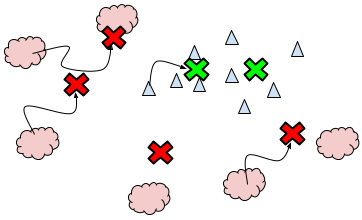
\includegraphics[width=0.6\linewidth]{Figures/anti-noising.png}
    \caption{Patterns with low bias (in red) are ignored as logits. In this way these patterns protect correct patterns with higher bias.}
\end{figure}

\noindent The architecture of the neural network is detailed:
\begin{itemize}
    \item \texttt{ConvHNN2d} with $9$ patterns and $5\times5$ kernel size and a \texttt{SiLU} activation
    \item \texttt{AutoEncoder} with: a linear convolution of $9$ channels to $3$ channels and $3\times3$ kernel size as encoder, a transposed convolution of $9$ channels to $2$ channels and $3\times3$ kernel size as decoder.
    \item Transpose convolution with Hopfield parameters.
\end{itemize}
This neural network was trained to reconstruct images, so its input was an image with Gaussian noise (with variance $1.0$). After training $20$ epochs, the MSE loss over the test set is $4 \times 10^{-2}$ with only $742$ trainable parameters.

\noindent Now we see how this neural network cleans up the images. In \cref{fig:CNNexample} we show the evolution of an image through the neural network.
\begin{figure}[htbp]
    \centering
    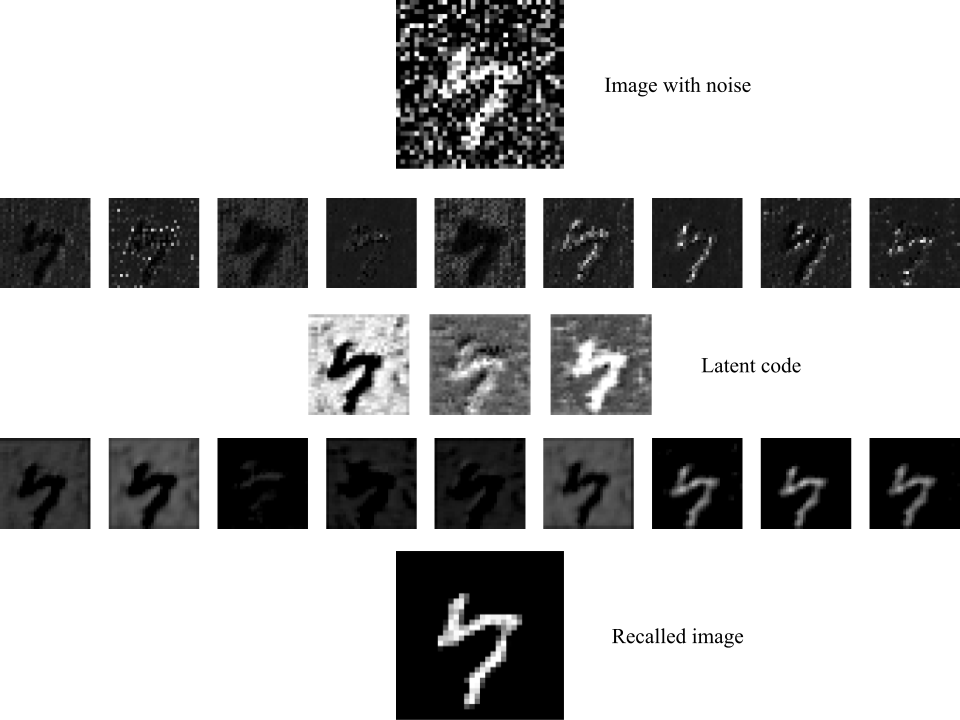
\includegraphics[width=1.0\linewidth]{Figures/CNNexample.png}
    \caption{Above is an image from MNIST with Gaussian noise (variance: $1.44$). The Hopfield convolution layer highlights certain patterns in the image (see white pixels). A linear CNN finds $3$ patterns from logits. An activation function then removes the residual noise so that a transposed CNN reconstructs the logits of the Hopfield convolution. Finally, the patterns from the Hopfield convolution are used to reconstruct the original image without noise.}
    \label{fig:CNNexample}
\end{figure}

\section{Variational Hopfield Neural Network (VHNN)}
In \cref{fig:VAE} we showed the architecture of the Variation Hopfield Neural Network, we observe that the number of samples defines the incidence of noise. If we get a single sample from the distribution $p$ we will have maximum noise, if we get a lot of samples the neural network will look like a typical Hopfield neural network.

\noindent We observe that $p = \mathbb{E}_p\left[M^n\right]$ where $M^n$ is the estimated distribution from $n$ Bernoulli samples from the distribution $p$. Let $M^n_k$ be the $k$th estimate associated with the $k$th sample (or the $k$th component of the softmax operation) and $\sigma_k$ be the variance of the Bernoulli sample from the $k$th component.
\[
\frac{M_k^n - p_k}{\sigma_k / \sqrt{n}} = \frac{\frac{1}{n}\sum^n \text{Be}(p_k) - p_k}{\sigma_k / \sqrt{n}} \overset{D}{\to} \mathcal{N}\left(0,1\right)\,,\quad \quad \sigma^2 = \text{Var}\left[\text{Be}(p_k)\right] = p_k(1-p_k)
\]
We can reformulate the noise with an approximation:
\[
S^\eta \mathdef p + \text{diag}\left(\sqrt{p_k(1-p_k)}\right)\varepsilon\,, \quad \quad \varepsilon \sim \mathcal{N}\left(0,\eta^2\mathds{1}\right)\,,\quad \eta\in\mathbb{R}_+
\]
where $S^\eta$ is the sampled data from the distribution $p$ in \textbf{VHNN}. Note that the noise $\eta$ is a continuous and eventually trainable value that replaces the iper parameter $\frac{1}{\sqrt{n}}$.

\noindent This formulation is very similar to the common formulation of VAE, which uses normal samples from the mean and variance given by the encoder.

\noindent In algorithm \ref{alg:VHNN_forward} we show the forward pass of layer VHNN.

\begin{lstlisting}[style=code, label=alg:VHNN_forward, caption=VHNN forward pass, language=Python]
import torch
from torch import nn
from torch.nn import functional

""" method of ConvHNN2d
attributes:
    channels, features, neurons: int
        positive values
    iterations: int
        number of neurons of theoretical Hopfield neural network
    _logbeta, _lognoise: nn.Parameter
        with shape (channels,)
    _patterns: nn.Parameter
        with shape (channels, features, neurons)
"""
def forward(self, x: torch.Tensor) -> torch.Tensor:

    # Shape of x must be (batch, channels, neurons)

    L = torch.exp(self._logbeta/2).view(-1, 1, 1) * self._patterns

    x = torch.exp(self._logbeta/2).view(1, -1, 1) * x
    for _ in range(self.iterations):
        x = torch.einsum('cfn, bcn -> bcf', L, x)
        x = nn.functional.softmax(x, dim=2)
        epsilon = torch.randn_like(x, device=x.device, requires_grad=False)
        xdet = x.detach().requires_grad(False)
        x = x + torch.exp(self._lognoise).view(1,-1,1) * (xdet*(1-xdet))**0.5 * epsilon
        x = torch.einsum('cfn, bcf -> bcn', L, x)

    x = torch.exp(-self._logbeta/2).view(1, -1, 1) * x
    return x
\end{lstlisting}

\paragraph{A Simple Experiment}
Using the noise, we study how the state evolution falls into and escapes from a $S_i$ (see \cref{prop:local_conv}).

\noindent Now we analyze the pattern set $S$ with $30$ patterns in the previously used $\mathbb{R}^{32\times32}$. We calculate the values $M$ and $\left(\Delta_i\right)_i$:
\[
M=\max_\mu \|x^\mu\| = 31.3933
\]
\[
\left(\Delta_i\right)_i=\left(\min_{j\neq i} (x^i)^Tx^i - (x^i)^Tx_j\right)_i = \text{ see \cref{tab:Delta}}
\]
\begin{table}[ht]
    \centering
    \begin{tabular}{|>{\columncolor{mint}}c||c|c|c|}
        \hline
        \rowcolor{lavender}
        digit     & pattern $1$ & pattern $2$ & pattern $3$ \\
        \hline
        $0$ & $88.0986$ & $80.1672$ & $131.736$ \\
        \hline
        $1$ & $53.4877$ & $69.0222$ & $59.4534$ \\
        \hline
        $2$ & $63.2126$ & $63.9695$ & $69.7267$ \\
        \hline
        $3$ & $65.0894$ & $55.4366$ & $46.0532$ \\
        \hline
        $4$ & $66.9539$ & $62.2354$ & $46.1037$ \\
        \hline
        $5$ & $41.8603$ & $39.9262$ & $37.5255$ \\
        \hline
        $6$ & $45.8450$ & $60.8577$ & $49.2501$ \\
        \hline
        $7$ & $55.7401$ & $51.3837$ & $35.1906$ \\
        \hline
        $8$ & $52.2477$ & $56.2899$ & $69.4982$ \\
        \hline
        $9$ & $107.129$ & $74.5176$ & $51.1973$ \\
        \hline
    \end{tabular}
    \caption{}
    \label{tab:Delta}
\end{table}

\noindent So we want to find a value $\beta$ such that
\[
    \forall i\left(\Delta_i\geq\frac{2}{\beta P} + \frac{1}{\beta}\log\left(2\left(P-1\right)P\beta M^2\right)\right)
\]
We calculate the minimum value $\Delta_{\min} = \min_i \Delta_i = 37.5255$ and simplify the equation:
\[
    \beta' \geq a + \log\beta'
\]
where: $\beta'=\beta\Delta_{\min}$, $a=\frac{2}{N}+\log\frac{2(N-1)NM^2}{\Delta_{\min}}$

\noindent If $a\leq1$ then the statement holds for any $\beta'$, otherwise we solve the equation $\beta'=a+\log\beta'$. The equation has solutions $\beta'_- < 1$ and $\beta'_+>1$.
We can use a fixed point iteration to find $\beta'_+$ with starting point $u_0=2a$ and $K$ iterations, so we know that $\beta = \frac{u_K}{\Delta_{\min}}$ is a good value for $\beta$, but we could choose a larger one. Now we can calculate the radius of each $S_i$: $R(S_i) \mathdef \frac{1}{\beta N M}$.

\noindent So we calculate $\beta = 0.0727$, but in this experiment we use $\beta=0.063$, which reduces the ability of the neural network to detect patterns. We set the noise to $\beta=0.3$ (high noise) so that we can see a change in opinion very quickly. The VHNN works over $4$ different states: for two patterns the noise does not allow an easy exit from local convergence, while for two patterns the neural network state jumps from one to the other. Empirically, with random inputs we have only these solutions, even if we start from a different $S_i$.

\noindent This is a stochastic process where the state of the neural network is a continuous distribution in the affine space of the patterns. In this way, the neural network can recall other patterns in a manner similar to a classical Markov chain. In a training process, the neural network can choose the position of the patterns to create a particular distribution, and the noise can take values that allow for fast training.

\begin{figure}[htbp]
    \centering
    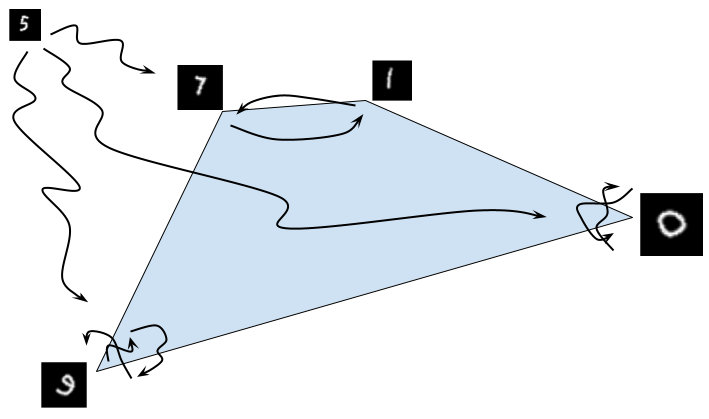
\includegraphics[width=0.6\linewidth]{Figures/VHNNdiagram.png}
    \label{fig:VHNNexample}
\end{figure}
